\documentclass{beamer}
\usepackage{siunitx}
\usepackage{physics}
\usepackage[demo]{graphicx}
\usepackage{caption}
\usepackage{subcaption}
\usepackage[utf8]{inputenc}

\usetheme{Warsaw}
\title{Speech Dereverberation based on Convex Optimization
Algorithms for Group Sparse Linear Prediction}
\author{JAYANT RANGI(MA17BTECH11006) \newline RITESH YADAV(MA17BTECH11009) }


\begin{document}

\maketitle 
\begin{frame}{Introduction : }
\textbf{Speech Dereverberation} has become an integral component of front end
processing techniques for \textbf{automatic speech recognition (ASR)}.
In particular, the recent advent of smart loudspeakers like the Amazon
Echo, Google Home, and Sonos One, has pushed the robustness
required in far-field ASR, as the user expects the same level of
performance in multiple condition, including being at different distances
in different acoustic environments.\textbf{This makes Dereverberation
one of the most prominent algorithm for enabling far-field
human-computer interaction.}
\newline
\begin{itemize}
    \item \textbf{Dereverberation} is the process by which the effects of reverberation(\textbf{i.e.} echo, resonance) are removed from sound. 
\end{itemize}

\end{frame}
\begin{frame}{Motivation : }
\centering
\begin{itemize}
    \item Speech dereverberation fundamental for enabling far-field \textbf{human computer} interaction, particularly with the recent advent of smart loudspeaker devices(\textbf{e.g.} Amazon echo, Apple siri).
    \begin{figure}

\begin{minipage}{.5\textwidth}
  \centering
  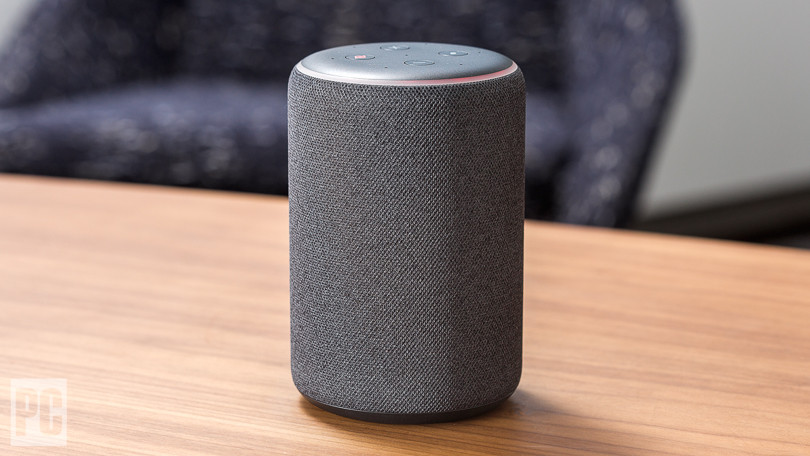
\includegraphics[width=.5\linewidth]{echo.jpg}
  \captionof{figure}{Amazon Echo}
  \label{fig:test1}
\end{minipage}%
\begin{minipage}{.5\textwidth}
  \centering
  
\includegraphics[width=.5\linewidth]{siri.jpg}
  \captionof{figure}{Apple Siri}
  \label{fig:test2}
\end{minipage}
\end{figure}
    
\end{itemize}
    
\end{frame}
\begin{frame}{Motivation : }
\begin{itemize}
    \item Blind methods based on multi-channel linear prediction (MCLP)
applied in the \textbf{STFT(Short Fourier Transform)}-domain particularly effective for the task:
\begin{itemize}
    \item no prior knowledge of the room acoustics,
    \item relatively easy and cheap to implement.
\newline
\end{itemize}

\item Popular MCLP-based methods look for a sparse desired speech
signal, assuming reverberation as a convolutive process (approximated
by the predicted speech) on a \textbf{STFT bin-by-bin basis}. This
is done by applying \textbf{nonconvex } algorithms.
\newline
\item We propose alternative formulations for sparse approximation
based on convex optimization
\end{itemize}
    
\end{frame}
\begin{frame}{Fundamentals : }
We consider an acoustic system composed of one speech point
source and M microphones. The signal at the \textit{m}-th microphone at
time n is :
\newline
\newline
$x_m(n)$ = \sum_{m=1}^{M}\textit{$r_m(n)$}$*$s(n) + $e_m(n)$
\newline
\newline
where \textit{s(n)} is the clean speech signal, $r_m(n)$ is the \textbf{RIR(Room Impulse Response)} between the speech source and the \textit{m}-th microphone, and $*$ is the convolution operator.
\end{frame}
\begin{frame}{Fundamentals : }
We focus our attention on so-called \textbf{utterance-based
batch processing} techniques where a full reverberant speech file is
processed all at once. Denoting \textit{s(k;n)} as the STFT of the
clean speech, with frame index n $\in$ (1,.....N) and frequency bin,
index k $\in$ (1,....K) the reverberant speech signal at the \textit{m}-th
microphone becomes :
\newline
\newline
$x_m(k,n)$ = \sum_{l=0}^{L_h-1}\textit{$h_m(k,l)$}$s(k,n-l) + e_m(k,n)$
\newline
\newline
where \textit{$h_m(k;l)$}  models the acoustic transfer function between the
speech source and the \textit{m}-th microphone in the \textit{k}-th frequency bin with length $L_h$.

\end{frame}
\begin{frame}{MCLP-based Dereverberation:}
The model divides the time-domain convolution into a set of convolution in the time-frequency domain
and has been widely adopted in the dereverberation literature.
Given the general assumption of ignoring the noise term, we can rewrite the equation as: \newline


    
\end{frame}
\begin{frame}{MCLP-based Dereverberation}
$x_m(k,n)=
\sum_{l=1}^{\tau-1}h_m(k,l)s(k,n-l) +
\sum_{l=\tau}^{L_g-1}h_m(k,l)s(k,n-l)
$ \newline
\begin{itemize}
    \item $n\in {1,....,N}$ frame index, $k \in {1,....,K}$ frequency bin index 
    \item s(k,n): clean speech
    \item $d_m(k,n)$: desired speech
    \item $r_m(k,n)$: reverberation term
    \item $h_m(k,l)$ Acoustic Transfer Function between the speech source and m-th microphone
    \item $\tau$: Delay to model direct speech and early reflections
    \item $L_g$: prediction order
\end{itemize}
    

    
\end{frame}

\begin{frame}{MCLP-based Dereverberation}
Desired speech signal using M predictors (order(L_g-1)): \newline \newline
d_m(k,n)=x_m(k,n)-\sum_{i=1}^{M}\sum_{l=0}^{L_g-1}x_i(k,n-\tau-l)g_m_,_i(k,l)
\newline \newline
$g_m_,_i$: l-th prediction coefficient between the i-th and the m-th channel \newline
    
\end{frame}
\begin{frame}{MCLP-based Dereverberation}
The equivalent model in matrix notation is:  \newline
$\textbf{D}(k)=\textbf{X}(k) - \textbf{X}_\tau(k)\textbf{G}(k)
 $ with   
 \begin{itemize}
     \item $\textbf{D}(k)=[d_1(k),...,d_m(k)]$
     \item $d_m(k)=[d_m(k,1),....d_m(k,N)]^T$
     \item $X(k)=[x_1(k),....x_M(k)]$
     \item $x_m(k)=[x_m(k,1),....x_m(k,N)]^T$
     \item $X_\tau(k)=[X_\tau_,_1(k),....,X_\tau_,_M(k)]$
     \item $G(k)=[g_1(k),....g_M(k)]$
     \item $g_m(k)=[g_m_,_1(k,0),....,g_m_,_1(k,L_g-1),....g_m_,_M(k,0),....,g_m_,_M(k,L_g-1)]^T$
     \item $X_\tau_,_m(k)$ is the convolution matrix of $x_m(k,n-\tau$
     \item The prediction matrix is $G(k)=[g_1(k),....,g_M(k)]$
     
 \end{itemize}
 
\end{frame}

\begin{frame}{Optimization}
\textbf{G}(k) is then found by solving the optimization problem: \newline \newline
$\DeclareUnicodeCharacter{}{\^G}= \underset{\textbf{G}}{\text{argmin}} || \textbf{X}-\textbf{X}_\tau\textbf{G}||^1_p_,_1 +
\alpha||\textbf{G}||^1_1_,_1 \newline 
$
\begin{itemize}
    \item For p=1 , equation is a element-wise regularized least-sum-of-absolute
    \item For p=2 , equation is a group LASSO problem
\end{itemize}

\end{frame}
\begin{frame}{Alternating Direction Method of Multipliers : }
\begin{itemize}
    \item A method :
    \newline
    \begin{itemize}
        \item with good robustness of method of multipliers
        \newline
        \item which can support decomposition
          \newline
    \end{itemize}
    \item \textbf{Decomposable method of multipliers}
\end{itemize}
\end{frame}
\begin{frame}{Alternating Direction Method of Multipliers :}
ADMM problem form (with f, g convex) :
\newline
\newline
 minimize      \textit{f(x) + g(x)}
 \newline
 subject to     A\textit{x} + B\textit{z} = \textit{c}
 \newline
 \newline
 – two sets of variables, with separable objective
 \newline
 $L_p(x,y,z)$ = \textit{f(x)+g(z)+$y^T$(Ax + Bz - c) + (\rho/2)||Ax + Bz -c||_2^2}
 \newline
 \newline
 \textbf{ADMM :}
 \newline
 $x^k^+^1$ := argmin_xL_p(x,z^k,y^k)
 \newline
 $z^k^+^1$ := argmin_zL_p(x^k^+^1,z,y^k)
 \newline
 $y^k^+^1$ := y^k + \rho(Ax^k^+^1 + Bz^k^+^1 - c)
    
\end{frame}
\begin{frame}{Alternating Direction Method of Multipliers :}
\begin{itemize}
    \item if we minimized over x and z jointly, reduces to method of multipliers
    \newline
    \item instead, we do one pass of a \textbf{Gauss-Seidel method}
    \newline
    \item we get splitting since we minimize over x with z fixed, and vice versa
\end{itemize}
    
\end{frame}
\begin{frame}{ADMM and Optimality conditions}
optimality conditions (for differentiable case): \newline
primal feasibility: Ax + Bz - c = 0 \newline
dual feasibility: $ $\nabla$f(x) + A^Ty = 0, $\nabla$g(z) + B^Ty = 0$ \newline
Since $z^k^+^1$ minimizes $L_p(x^k^+^1,z,y^k)$ \newline
0 = $ $\nabla$g(z^k^+^1) + B^Ty^k + $\rho$B^T(Ax^k^+^1+Bz^k^+^1-c) $ \newline
0 = $ $\nabla$g(z^k^+^1) + B^Ty^k^+^1 $ \newline
\newline
So, with ADMM dual variable update, $(x^k^+^1,z^k^+^1,y^k^+^1)$ satisfies second dual feasibility condition.\newline
Primal and first dual feasibility are achieved as k\rightarrow \infty \newline
 

    
\end{frame}
\begin{frame}{ADMM with scaled dual variables}
combine linear and quadratic terms in augmented Lagrangian \newline
$
L_p(x,y,z)=f(x)+g(z)+y^T(Ax+Bz-c)+(\rho/2)||Ax+Bz-c||^2_2 
 $  \newline
 $
L_p(x,y,z)=f(x)+g(z)+(\rho/2)||Ax+Bz-c||^2_2 
 $+ const. \newline
 with $u^k=(1/\rho)y^k$ \newline
 \newline
 ADMM (scaled dual form): \newline
 $x^k^+^1 := \underset{x}{\text{argmin}}(f(x)+(\rho/2)||Ax+Bz^k-c+u^k||^2_2) \newline
 $
  $z^k^+^1 := \underset{z}{\text{argmin}}(g(z)+(\rho/2)||Ax^k^+^1+Bz-c+u^k||^2_2) \newline
 $
 $u^k^+^1 := u^k+(Ax^k^+^1+Bz^k^+^1-c) $
 
\end{frame}
\begin{frame}{Sources : }
\begin{itemize}
    \item \textbf{SPEECH DEREVERBERATION BASED ON CONVEX OPTIMIZATION ALGORITHMS FOR GROUP SPARSE LINEAR PREDICTION}
\newline
Daniele $Giacobello^1$ and Tobias Lindstrom $Jensen^2$ \newline
\item \textbf{Alternating Direction Method of Multipliers}
\newline
Prof S. Boyd
EE364b, Stanford University
\newline
\end{itemize}
\end{frame}


\section{Introduction}

\end{document}